\documentclass{standalone}
\usepackage{tikz}
\usetikzlibrary{patterns, positioning}

\begin{document}
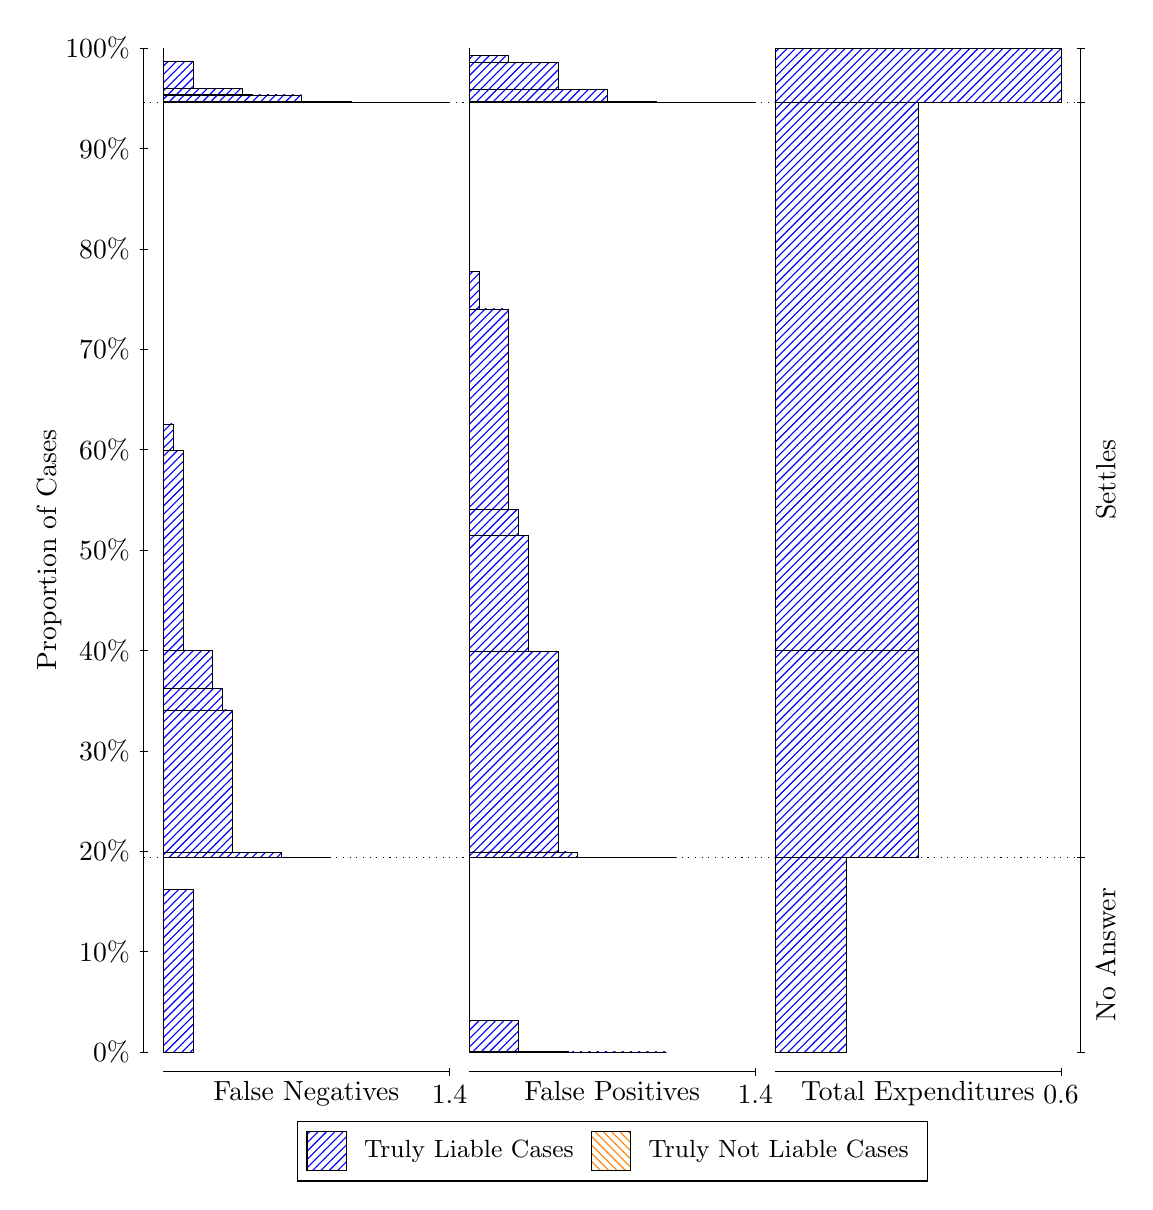
\begin{tikzpicture}
\draw[black, very thin] (1.5,1.75) -- (1.5,14.5);
\node[rotate=90, anchor=center] at (0.3, 8.125) {Proportion of Cases};
\draw[black, very thin] (1.45,1.75) -- (1.55,1.75);
\node[anchor=east] at (1.45, 1.75) {0\%};
\draw[black, very thin] (1.45,3.025) -- (1.55,3.025);
\node[anchor=east] at (1.45, 3.025) {10\%};
\draw[black, very thin] (1.45,4.3) -- (1.55,4.3);
\node[anchor=east] at (1.45, 4.3) {20\%};
\draw[black, very thin] (1.45,5.575) -- (1.55,5.575);
\node[anchor=east] at (1.45, 5.575) {30\%};
\draw[black, very thin] (1.45,6.85) -- (1.55,6.85);
\node[anchor=east] at (1.45, 6.85) {40\%};
\draw[black, very thin] (1.45,8.125) -- (1.55,8.125);
\node[anchor=east] at (1.45, 8.125) {50\%};
\draw[black, very thin] (1.45,9.4) -- (1.55,9.4);
\node[anchor=east] at (1.45, 9.4) {60\%};
\draw[black, very thin] (1.45,10.675) -- (1.55,10.675);
\node[anchor=east] at (1.45, 10.675) {70\%};
\draw[black, very thin] (1.45,11.95) -- (1.55,11.95);
\node[anchor=east] at (1.45, 11.95) {80\%};
\draw[black, very thin] (1.45,13.225) -- (1.55,13.225);
\node[anchor=east] at (1.45, 13.225) {90\%};
\draw[black, very thin] (1.45,14.5) -- (1.55,14.5);
\node[anchor=east] at (1.45, 14.5) {100\%};

\draw[black, very thin] (13.4,1.75) -- (13.4,14.5);
\draw[black, very thin] (13.35,1.75) -- (13.45,1.75);
\node[anchor=west] at (13.35, 1.75) {};
\draw[black, very thin] (13.35,4.2242) -- (13.45,4.2242);
\node[anchor=west] at (13.35, 4.2242) {};
\draw[black, very thin] (13.35,13.811) -- (13.45,13.811);
\node[anchor=west] at (13.35, 13.811) {};
\draw[black, very thin] (13.35,14.5) -- (13.45,14.5);
\node[anchor=west] at (13.35, 14.5) {};

\draw[black, very thin, pattern color=blue, pattern=north east lines] (1.75,1.75) rectangle (2.1259,3.8191);
\draw[black, very thin, pattern color=orange, pattern=north west lines] (1.75,3.8191) rectangle (1.75,3.8191);
\draw[black, very thin, pattern color=blue, pattern=north east lines] (1.75,3.8191) rectangle (1.75,4.2242);
\draw[black, very thin, pattern color=blue, pattern=north east lines] (1.75,4.2242) rectangle (3.8799,4.2242);
\draw[black, very thin, pattern color=blue, pattern=north east lines] (1.75,4.2242) rectangle (3.2534,4.2886);
\draw[black, very thin, pattern color=blue, pattern=north east lines] (1.75,4.2886) rectangle (3.1282,4.2894);
\draw[black, very thin, pattern color=blue, pattern=north east lines] (1.75,4.2894) rectangle (2.627,6.0944);
\draw[black, very thin, pattern color=blue, pattern=north east lines] (1.75,6.0944) rectangle (2.5017,6.3714);
\draw[black, very thin, pattern color=blue, pattern=north east lines] (1.75,6.3714) rectangle (2.3764,6.8474);
\draw[black, very thin, pattern color=blue, pattern=north east lines] (1.75,6.8474) rectangle (2.0006,9.3905);
\draw[black, very thin, pattern color=blue, pattern=north east lines] (1.75,9.3905) rectangle (1.8753,9.728);
\draw[black, very thin, pattern color=orange, pattern=north west lines] (1.75,9.728) rectangle (1.75,9.728);
\draw[black, very thin, pattern color=blue, pattern=north east lines] (1.75,9.728) rectangle (1.75,13.811);
\draw[black, very thin, pattern color=blue, pattern=north east lines] (1.75,13.811) rectangle (5.3833,13.811);
\draw[black, very thin, pattern color=blue, pattern=north east lines] (1.75,13.811) rectangle (4.7569,13.811);
\draw[black, very thin, pattern color=blue, pattern=north east lines] (1.75,13.811) rectangle (4.1305,13.827);
\draw[black, very thin, pattern color=blue, pattern=north east lines] (1.75,13.827) rectangle (3.504,13.906);
\draw[black, very thin, pattern color=blue, pattern=north east lines] (1.75,13.906) rectangle (3.3787,13.906);
\draw[black, very thin, pattern color=blue, pattern=north east lines] (1.75,13.906) rectangle (2.8776,13.908);
\draw[black, very thin, pattern color=blue, pattern=north east lines] (1.75,13.908) rectangle (2.7523,13.989);
\draw[black, very thin, pattern color=blue, pattern=north east lines] (1.75,13.989) rectangle (2.2511,13.989);
\draw[black, very thin, pattern color=blue, pattern=north east lines] (1.75,13.989) rectangle (2.1259,14.333);
\draw[black, very thin, pattern color=orange, pattern=north west lines] (1.75,14.333) rectangle (1.75,14.333);
\draw[black, very thin, pattern color=blue, pattern=north east lines] (1.75,14.333) rectangle (1.75,14.5);
\draw[black, very thin, pattern color=orange, pattern=north west lines] (5.6333,1.75) rectangle (8.1391,1.75);
\draw[black, very thin, pattern color=blue, pattern=north east lines] (5.6333,1.75) rectangle (8.1391,1.75);
\draw[black, very thin, pattern color=blue, pattern=north east lines] (5.6333,1.75) rectangle (7.5126,1.75);
\draw[black, very thin, pattern color=blue, pattern=north east lines] (5.6333,1.75) rectangle (6.8862,1.7535);
\draw[black, very thin, pattern color=blue, pattern=north east lines] (5.6333,1.7535) rectangle (6.2598,2.1551);
\draw[black, very thin, pattern color=blue, pattern=north east lines] (5.6333,2.1551) rectangle (5.6333,4.2242);
\draw[black, very thin, pattern color=orange, pattern=north west lines] (5.6333,4.2242) rectangle (8.2644,4.2242);
\draw[black, very thin, pattern color=blue, pattern=north east lines] (5.6333,4.2242) rectangle (8.2644,4.2242);
\draw[black, very thin, pattern color=blue, pattern=north east lines] (5.6333,4.2242) rectangle (7.6379,4.2242);
\draw[black, very thin, pattern color=orange, pattern=north west lines] (5.6333,4.2242) rectangle (7.5126,4.2242);
\draw[black, very thin, pattern color=blue, pattern=north east lines] (5.6333,4.2242) rectangle (7.5126,4.2242);
\draw[black, very thin, pattern color=blue, pattern=north east lines] (5.6333,4.2242) rectangle (7.0115,4.2879);
\draw[black, very thin, pattern color=blue, pattern=north east lines] (5.6333,4.2879) rectangle (6.8862,4.2913);
\draw[black, very thin, pattern color=orange, pattern=north west lines] (5.6333,4.2913) rectangle (6.7609,4.2913);
\draw[black, very thin, pattern color=blue, pattern=north east lines] (5.6333,4.2913) rectangle (6.7609,6.8413);
\draw[black, very thin, pattern color=blue, pattern=north east lines] (5.6333,6.8413) rectangle (6.3851,8.3076);
\draw[black, very thin, pattern color=blue, pattern=north east lines] (5.6333,8.3076) rectangle (6.2598,8.6451);
\draw[black, very thin, pattern color=blue, pattern=north east lines] (5.6333,8.6451) rectangle (6.1345,11.188);
\draw[black, very thin, pattern color=blue, pattern=north east lines] (5.6333,11.188) rectangle (5.7586,11.664);
\draw[black, very thin, pattern color=blue, pattern=north east lines] (5.6333,11.664) rectangle (5.6333,13.811);
\draw[black, very thin, pattern color=orange, pattern=north west lines] (5.6333,13.811) rectangle (9.2667,13.811);
\draw[black, very thin, pattern color=blue, pattern=north east lines] (5.6333,13.811) rectangle (9.2667,13.811);
\draw[black, very thin, pattern color=orange, pattern=north west lines] (5.6333,13.811) rectangle (8.6402,13.811);
\draw[black, very thin, pattern color=blue, pattern=north east lines] (5.6333,13.811) rectangle (8.6402,13.811);
\draw[black, very thin, pattern color=orange, pattern=north west lines] (5.6333,13.811) rectangle (8.0138,13.811);
\draw[black, very thin, pattern color=blue, pattern=north east lines] (5.6333,13.811) rectangle (8.0138,13.819);
\draw[black, very thin, pattern color=blue, pattern=north east lines] (5.6333,13.819) rectangle (7.3874,13.978);
\draw[black, very thin, pattern color=blue, pattern=north east lines] (5.6333,13.978) rectangle (6.7609,14.322);
\draw[black, very thin, pattern color=orange, pattern=north west lines] (5.6333,14.322) rectangle (6.6356,14.322);
\draw[black, very thin, pattern color=blue, pattern=north east lines] (5.6333,14.322) rectangle (6.6356,14.322);
\draw[black, very thin, pattern color=blue, pattern=north east lines] (5.6333,14.322) rectangle (6.1345,14.404);
\draw[black, very thin, pattern color=blue, pattern=north east lines] (5.6333,14.404) rectangle (6.0092,14.405);
\draw[black, very thin, pattern color=orange, pattern=north west lines] (5.6333,14.405) rectangle (6.0092,14.405);
\draw[black, very thin, pattern color=blue, pattern=north east lines] (5.6333,14.405) rectangle (6.0092,14.405);
\draw[black, very thin, pattern color=blue, pattern=north east lines] (5.6333,14.405) rectangle (5.6333,14.5);
\draw[black, very thin, pattern color=orange, pattern=north west lines] (9.5167,1.75) rectangle (10.425,1.75);
\draw[black, very thin, pattern color=blue, pattern=north east lines] (9.5167,1.75) rectangle (10.425,4.2242);
\draw[black, very thin, pattern color=orange, pattern=north west lines] (9.5167,4.2242) rectangle (11.333,4.2242);
\draw[black, very thin, pattern color=blue, pattern=north east lines] (9.5167,4.2242) rectangle (11.333,6.8488);
\draw[black, very thin, pattern color=orange, pattern=north west lines] (9.5167,6.8488) rectangle (11.333,6.8488);
\draw[black, very thin, pattern color=blue, pattern=north east lines] (9.5167,6.8488) rectangle (11.333,13.811);
\draw[black, very thin, pattern color=orange, pattern=north west lines] (9.5167,13.811) rectangle (13.15,13.811);
\draw[black, very thin, pattern color=blue, pattern=north east lines] (9.5167,13.811) rectangle (13.15,14.5);
\draw[black, dotted] (1.5,4.2242) -- (13.4,4.2242);
\draw[black, dotted] (1.5,13.811) -- (13.4,13.811);
\draw[black, very thin] (1.75,1.5) -- (5.3833,1.5);
\node[anchor=north] at (3.5667, 1.5) {False Negatives};
\draw[black, very thin] (5.3833,1.45) -- (5.3833,1.55);
\node[anchor=north] at (5.3833, 1.45) {1.4};

\draw[black, very thin] (5.6333,1.5) -- (9.2667,1.5);
\node[anchor=north] at (7.45, 1.5) {False Positives};
\draw[black, very thin] (9.2667,1.45) -- (9.2667,1.55);
\node[anchor=north] at (9.2667, 1.45) {1.4};

\draw[black, very thin] (9.5167,1.5) -- (13.15,1.5);
\node[anchor=north] at (11.333, 1.5) {Total Expenditures};
\draw[black, very thin] (13.15,1.45) -- (13.15,1.55);
\node[anchor=north] at (13.15, 1.45) {0.6};

\node[black, centered, rotate=90] at (13.72, 2.9871) {No Answer};
\node[black, centered, rotate=90] at (13.72, 9.0178) {Settles};


\draw (7.449999999999999,1.5) node[draw=none] (baseCoordinate) {};
\begin{scope}[align=center]
        \matrix[scale=0.5, draw=black, below=0.5cm of baseCoordinate, nodes={draw}, column sep=0.1cm]{
            \node[rectangle, draw, minimum width=0.5cm, minimum height=0.5cm, pattern=north east lines, pattern color=blue] {}; &
            \node[draw=none, font=\small] (B) {Truly Liable Cases}; &
            \node[rectangle, draw, minimum width=0.5cm, minimum height=0.5cm, pattern=north west lines, pattern color=orange] {}; &
            \node[draw=none, font=\small] (B) {Truly Not Liable Cases}; \\
            };
\end{scope}

\end{tikzpicture}
\end{document}